\documentclass[t]{beamer}
\usepackage[utf8]{inputenc}  % to be able to type unicode text directly
%\usepackage[french]{babel}   % french typographical conventions
\usepackage{inconsolata}     % for a nicer (e.g. non-courier) tt family font
%\usepackage{amsthm,amsmath}  % fancier mathematics
\usepackage{array} % to fine-tune tabular spacing
\usepackage{bbm} % for blackboard 1

\usepackage{graphicx}        % to include images
%\usepackage{animate}         % to include animated images
\usepackage{soul}            % for colored strikethrough
%\usepackage{bbding}          % for Checkmark and XSolidBrush
\usepackage{hyperref,url}

\colorlet{darkgreen}{black!50!green}  % used for page numbers
\definecolor{term}{rgb}{.9,.9,.9}     % used for code insets

\setlength{\parindent}{0em}
\setlength{\parskip}{1em}


% coco's macros
\def\R{\mathbf{R}}
\def\F{\mathcal{F}}
\def\x{\mathbf{x}}
\def\y{\mathbf{y}}
\def\u{\mathbf{u}}
\def\Z{\mathbf{Z}}
\def\d{\mathrm{d}}
\DeclareMathOperator*{\argmin}{arg\,min}
\DeclareMathOperator*{\argmax}{arg\,max}
\newcommand{\reference}[1] {{\scriptsize \color{gray}  #1 }}
\newcommand{\referencep}[1] {{\tiny \color{gray}  #1 }}
\newcommand{\unit}[1] {{\tiny \color{gray}  #1 }}

% disable spacing around verbatim
\usepackage{etoolbox}
\makeatletter\preto{\@verbatim}{\topsep=0pt \partopsep=0pt }\makeatother

% disable headings, set slide numbers in green
\mode<all>\setbeamertemplate{navigation symbols}{}
\defbeamertemplate*{footline}{pagecount}{\leavevmode\hfill\color{darkgreen}
   \insertframenumber{} / \inserttotalframenumber\hspace*{2ex}\vskip0pt}

%% select red color for strikethrough
\makeatletter
\newcommand\SoulColor{%
  \let\set@color\beamerorig@set@color
  \let\reset@color\beamerorig@reset@color}
\makeatother
\newcommand<>{\St}[1]{\only#2{\SoulColor\st{#1}}}
\setstcolor{red}

% make everything monospace
\renewcommand*\familydefault{\ttdefault}

\begin{document}

\begin{frame}
IMAGE PROCESSING WITH GRAPHS\hfill{\footnotesize{\color{gray}enric meinhardt-llopis}}\\
============================

\vfill

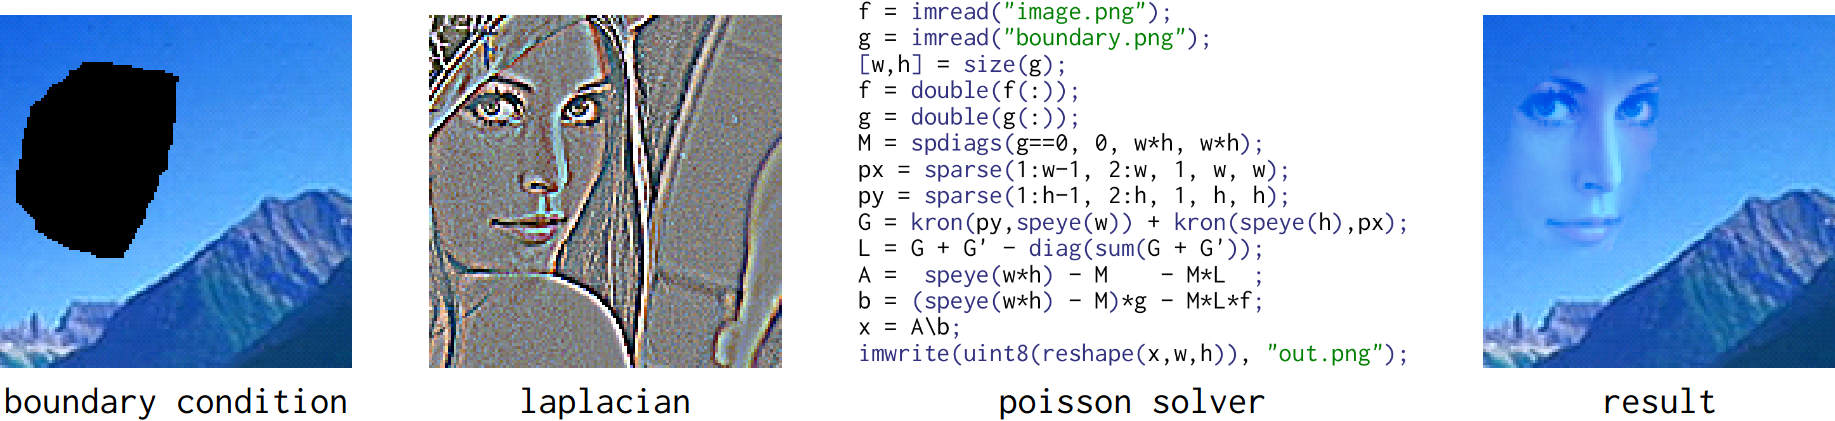
\includegraphics[width=0.9\linewidth]{lenashot.png}

\vfill
{\bf Before mlbriefs}:
a 10-page notebook with many experiments over the same example image

{\bf After mlbriefs}: 
an ``IPOL notebook'' where you can change the input image and re-run the experiments

1. Construction of the grid graph {\color{gray}\small(kronecker product)}\\
2. Morphological operators {\color{gray}\small (erosion, gradients, ...)}\\
3. Local linear operators {\color{gray}\small(grad, div, lap, hess, ...)}\\
4. Linear discrete PDE on graphs\\
{\color{gray}$\quad\ $\small(diffusion, Poisson, Helmholtz, Schrödinger, ...)}

\end{frame}


\begin{frame}
IMAGE PROCESSING WITH GRAPHS\hfill{\footnotesize{\color{gray}enric meinhardt-llopis}}
%\\
%============================

{\bf Goal:} Show the graph matrices acting over the image data.

- Adjacency matrix : mathematical morphology\\
- Incidence matrix : first derivatives\\
- Laplacian matrix : second derivatives

\begin{tabular}{ccc}
	\includegraphics[width=0.3\linewidth]{f/x_binarized.png}&
	\includegraphics[width=0.3\linewidth]{f/x_6_morphogray.png}&
	\includegraphics[width=0.3\linewidth]{f/x_6_median.png}\\
	{\tt x} & {\tt A**6 @ x} & {\tt (A**6 @ x)>M/2} \\
	\includegraphics[width=0.3\linewidth]{f/x_6_erosion.png}&
	\includegraphics[width=0.3\linewidth]{f/x_6_dilation.png}&
	\includegraphics[width=0.3\linewidth]{f/x_igradient.png}\\
	{\tt (A**6 @ x)>0} & {\tt (A**6 @ x)>=M} & morpho-gradient \\
\end{tabular}

\end{frame}

\begin{frame}
EXAMPLE OF A COMPLETE CELL AND ITS RESULT\\
=========================================

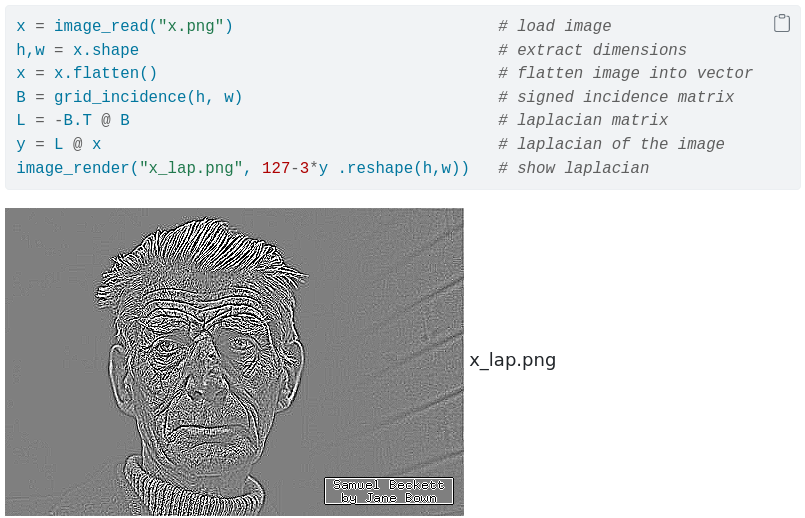
\includegraphics[width=\textwidth]{vxlap.png}
\end{frame}

\begin{frame}
CODE, ARTICLE AND DEMO ON THE SAME TEXT FILE\\
============================================

\vfill

%\begin{tabular}{lll}
%	{\tt a.py} (source) &
%	{\tt a.ipynb} (generated) &
%	{\tt a.html} (generated) \\
%	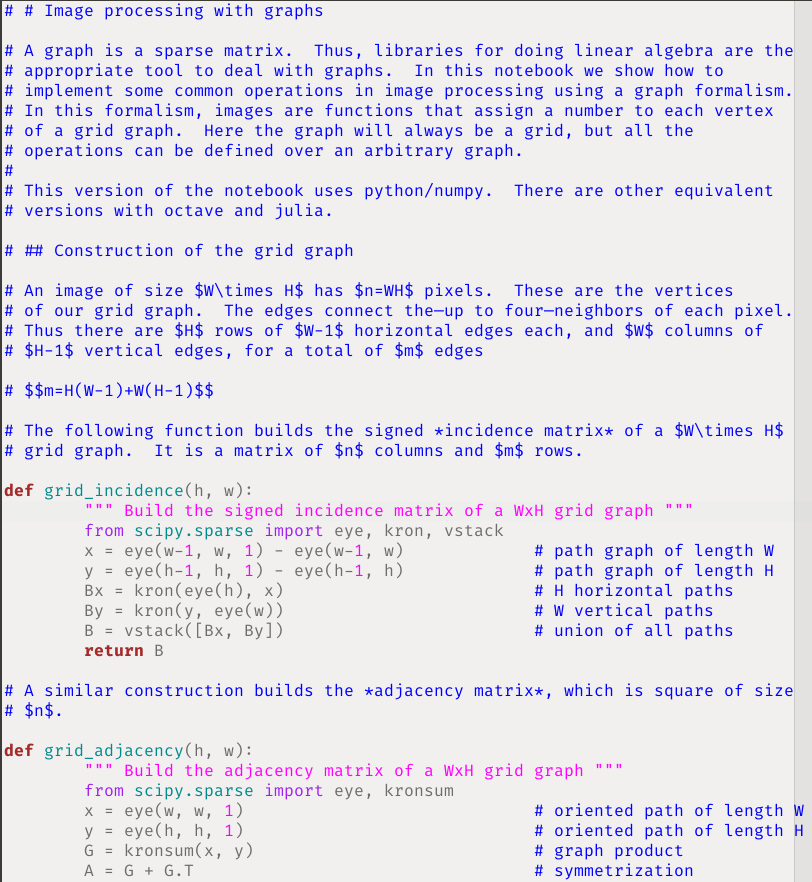
\includegraphics[width=0.33\linewidth]{apy.png}&
%	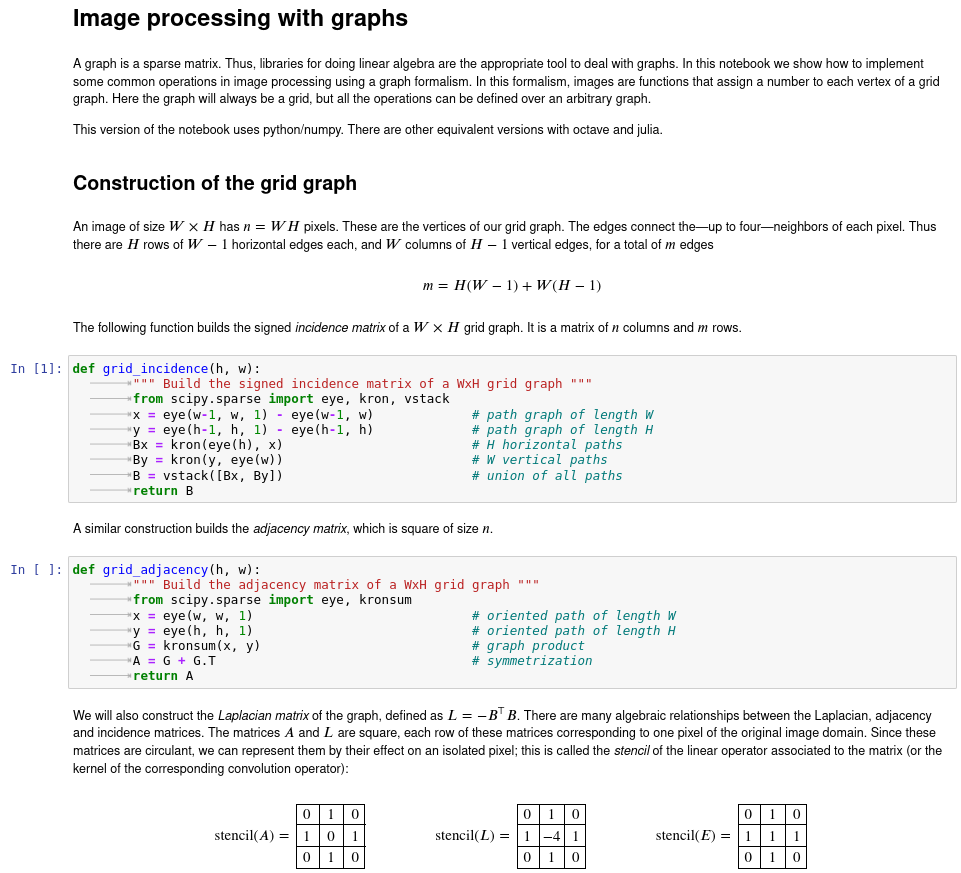
\includegraphics[width=0.33\linewidth]{aipynb.png}&
%	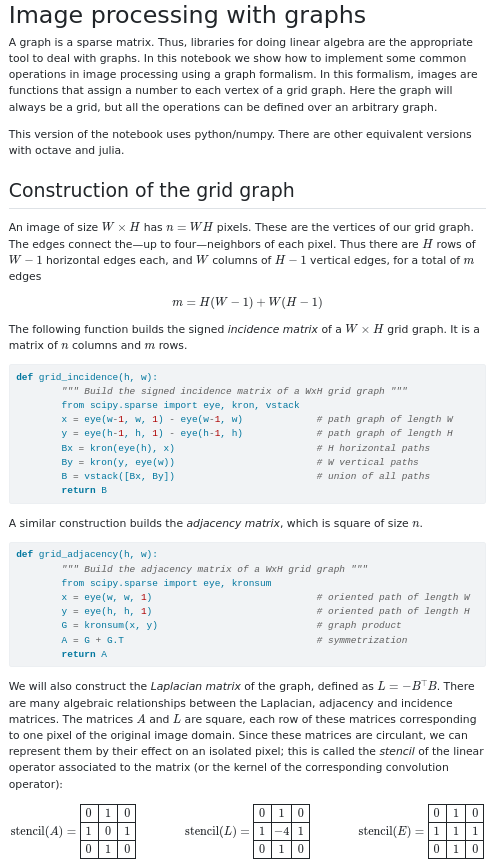
\includegraphics[width=0.33\linewidth]{ahtml.png}
%\end{tabular}
\begin{columns}
	\begin{column}{0.33\textwidth}
	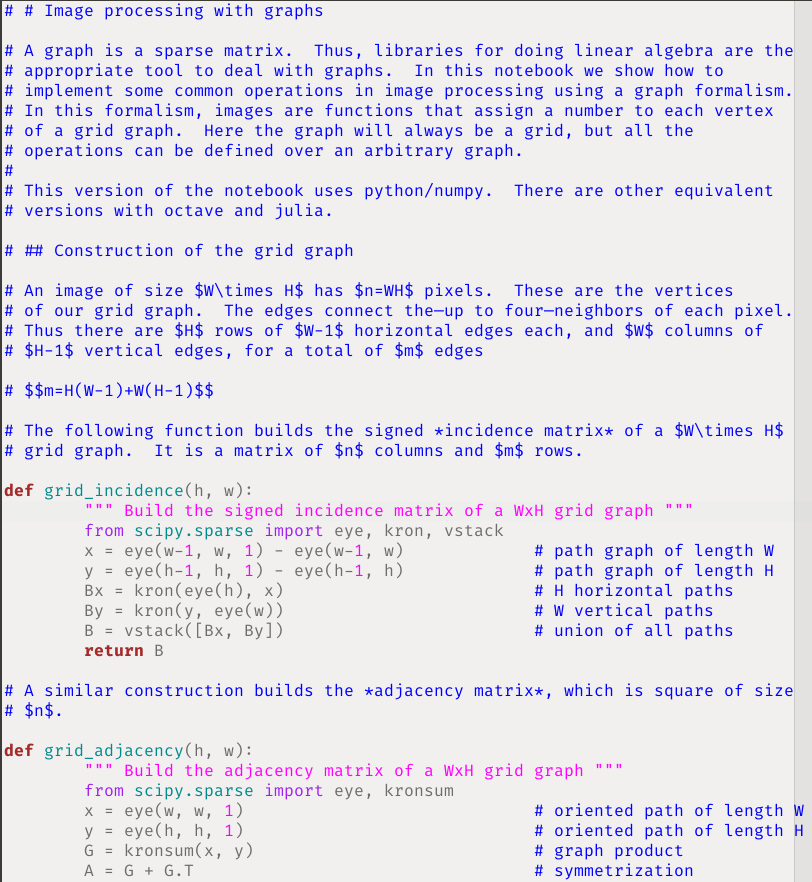
\includegraphics[width=\linewidth]{apy.png}\\
	\small{\tt a.py} (source)
	\end{column}

	\begin{column}{0.33\textwidth}
	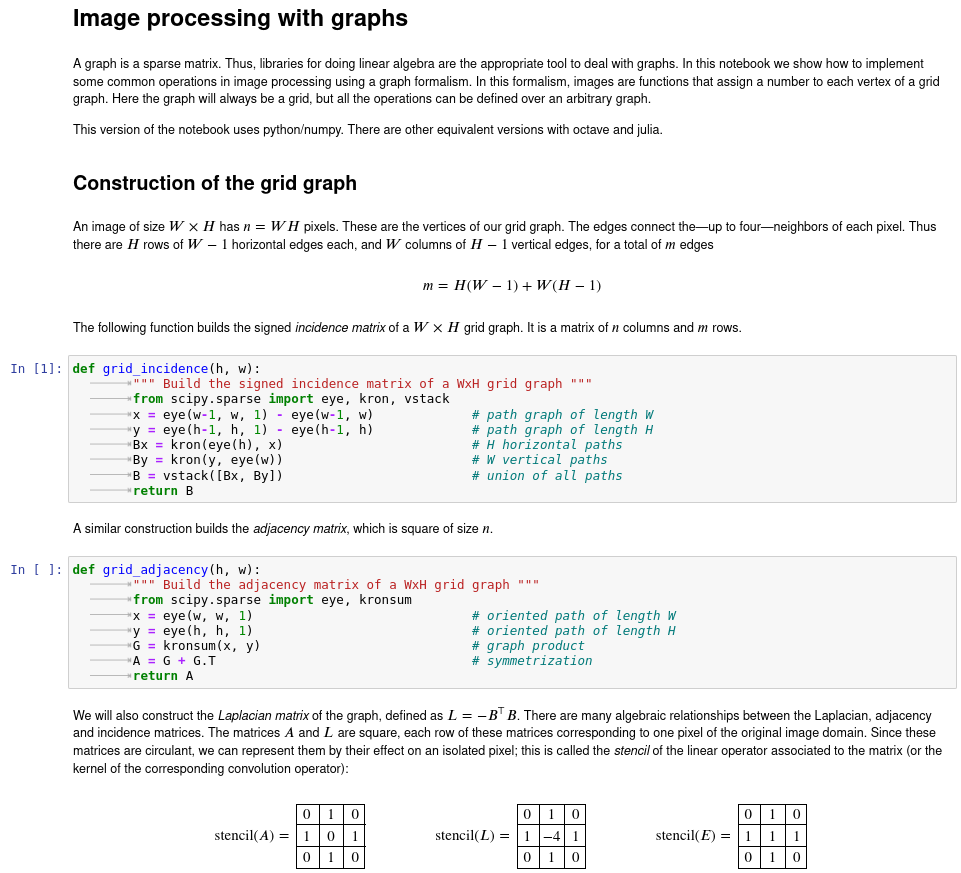
\includegraphics[width=\linewidth]{aipynb.png}\\
	\small{\tt a.ipynb} (generated)
	\end{column}

	\begin{column}{0.33\textwidth}
	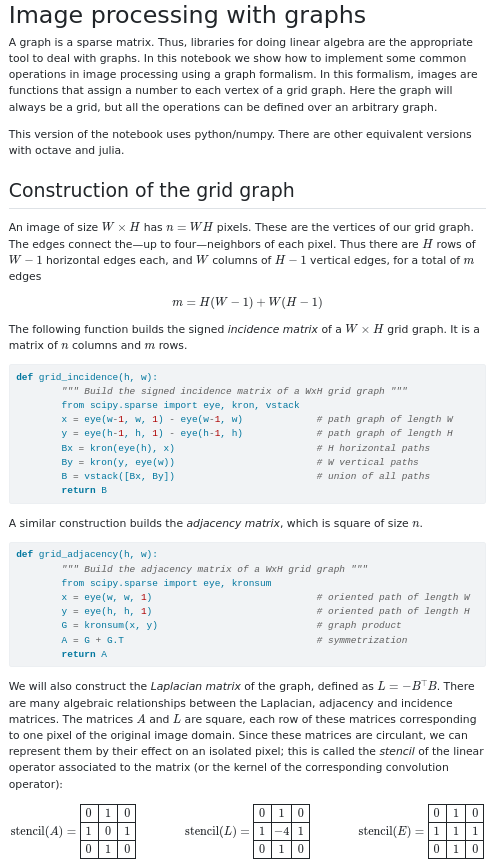
\includegraphics[width=\linewidth]{ahtml.png}
	\small{\tt a.html} (generated)
	\end{column}
\end{columns}

\end{frame}



\end{document}


% vim:sw=2 ts=2 spell spelllang=fr:
